

\subsubsection{Website}
\noindent Um zu verstehen wie die Interaktion zwischen Nutzer und System funktioniert, ist es notwendig die Kommunikation der einzelnen Komponenten, die zuständig für das Generieren des UI sind, näher zu beleuchten. 
Besonders geeignet hierfür ist das Model-View-Controller (MVC) Pattern. 
Im folgenden wird zunächst genauer auf das Erzeugen der UI, in unserem Fall eine Website und anschließend auf die Einbindung einzelner Darstellungskomponenten in dieses eingegangen. \\

\begin{figure}[h]
\centering
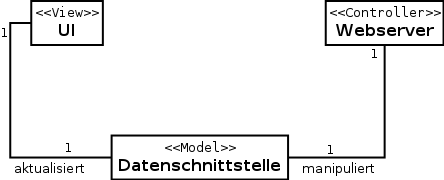
\includegraphics[width=1.0\linewidth]{Grafik/Diagramm/Pattern/MVC/Website/Kontextdiagramm.png}
\caption[MVC Website Klassen]{MVC-Pattern zum Website anzeigen}
\end{figure}

\noindent  Das UI ist der für den Benutzer sichtbare Teil des Systems. Betätigt der Nutzer in diesem eine Schaltfläche, so werden seine Eingaben durch den Webserver ausgewertet und an die entsprechenden Instanzen im System weitergeleitet. Sollen in etwa benutzerbezogene Daten abgefragt werden, so greift der Webserver auf die Datenschnittstelle zu, die die entsprechenden Daten über eine SPARQL Anfragen an die RDF-Datenbank bereitstellt. Auf Basis dieser Rückgabe generiert der Webserver nun das entsprechende UI und  zeigt dieses dem Nutzer an.
Sollten sich die Daten in der Datenbank ändern, so registriert die Datenschnittstelle dies und informiert das UI hierüber, damit die Anzeige entsprechend verändert wird.


\begin{figure}[h]
\centering
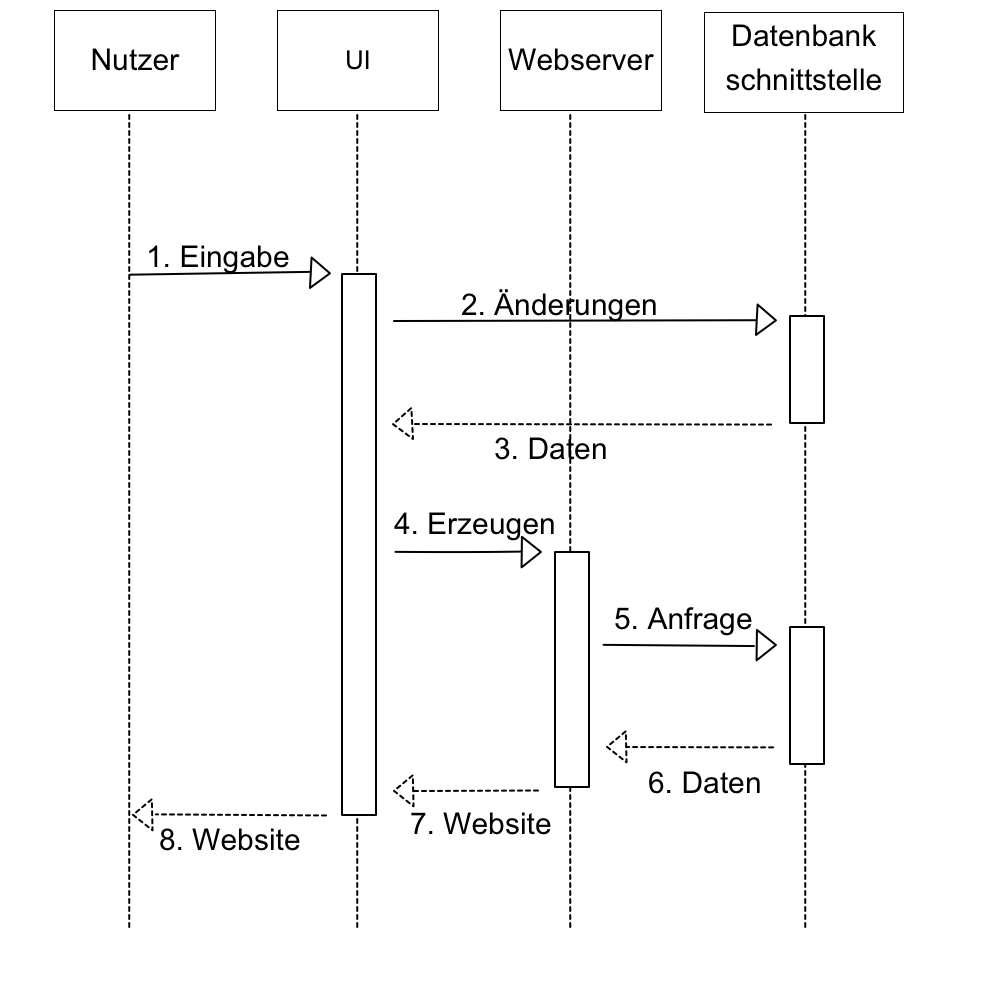
\includegraphics[width=0.6\linewidth]{Grafik/Diagramm/Pattern/MVC/Website/Sequenzdiagramm.png}
\caption[MVC Website Sequenz]{MVC-Pattern Sequenz zum Generieren der Website}
\end{figure}


\clearpage

\subsubsection{Plugin}
Um nun bestimmte Darstellungskomponenten, im weiteren als Plugins bezeichnet, in das UI einzubinden wird das MVC-Pattern erneut verwendet. Solche Plugins können z.B. die Ausgabe von Ergebnissen als Text oder Grafik sein, aber auch Eingabemasken zum Erstellen von Modellen.


\begin{figure}[h]
\centering
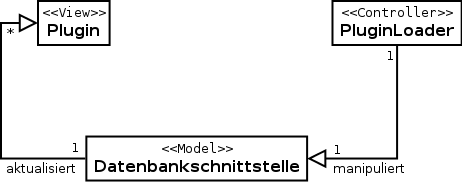
\includegraphics[width=1.0\linewidth]{Grafik/Diagramm/Pattern/MVC/Plugin/Kontextdiagramm.png}
\caption[MVC Website Klassen]{MVC-Pattern zum Website anzeigen}
\end{figure}

\noindent Sollte der Benutzer z.B. ein Modell generieren wollen oder sich ein Ergebnis anzeigen lassen, so formuliert der PluginLoader eine Anfrage an die Datenschnittstelle um mögliche Änderungen an diese zu senden. Nach diesem Aktualisierungsprozess wird ein Plugin durch den PluginLoader generiert, das über die Datenschnittstelle die notwendigen Informationen bezieht. Sollten hierbei Anfragen an andere Server nötig sein, so werden diese ebenfalls von der Datenschnittstelle mittels des REST-Protokolls durchgeführt. 
Das fertige Plugin wird nun in das Haupt-UI integriert.


\begin{figure}[h]
\centering
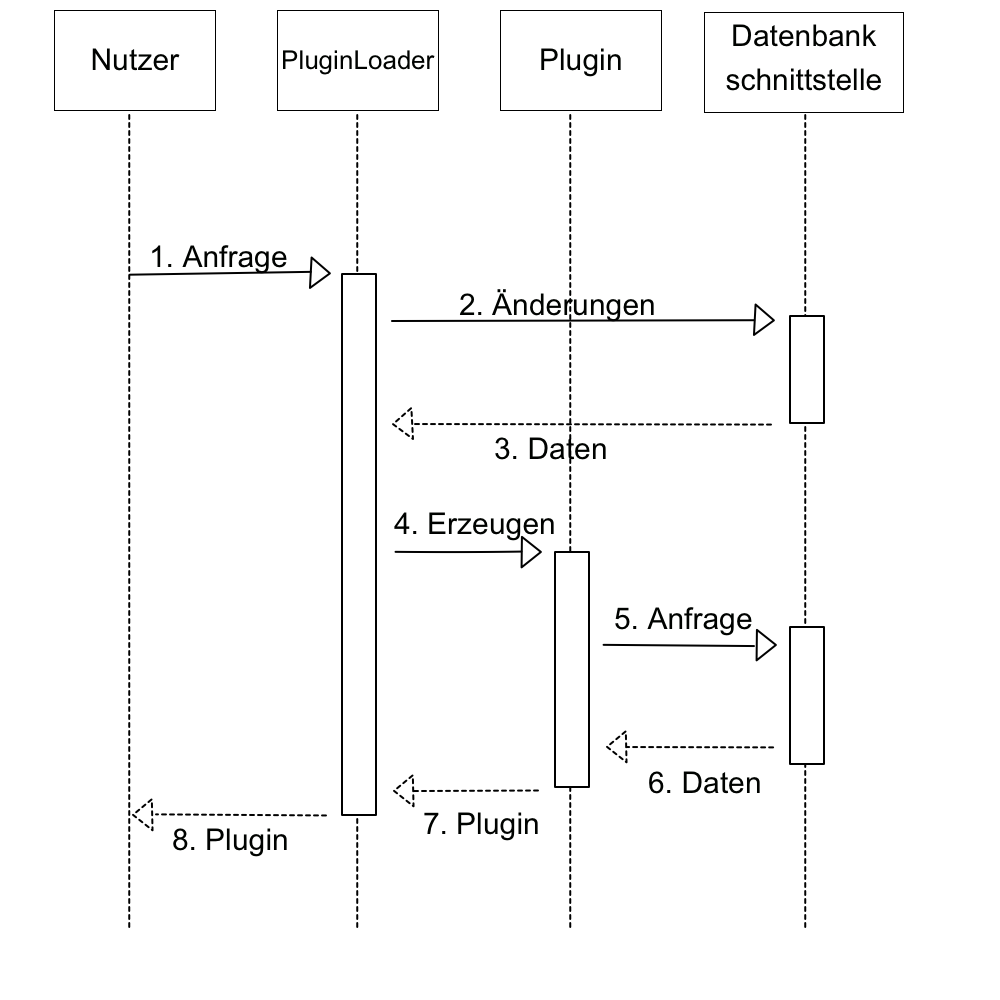
\includegraphics[width=1.0\linewidth]{Grafik/Diagramm/Pattern/MVC/Plugin/Sequenzdiagramm.png}
\caption[MVC Website Sequenz]{MVC-Pattern Sequenz zum Generieren der Website}
\end{figure}

\clearpage

\subsubsection{Was spricht für Model-View-Controller?}
Das MVC-Pattern ermöglicht es das System leicht zu erweitern. Durch die Anwendung des Pattern zur Erzeugung des UI, wird es leicht dieses auszutauschen. Zum Einbinden einer mobilen Website oder einer Desktopoberfläche genügt es lediglich das UI Objekt zu ändern. Letzteres würde allerdings einen Mehraufwand erfordern, da die grafische Implementierung auf Seiten des Client erfolgen müsste.
Durch die Einbindung verschiedener Plugins in das System, wird gewährleistet, das auf neue Gegebenheiten schnell reagiert werden kann.
Sollte z.B. ein Algorithmus eine spezifische Ausgabe benötigen, könnte speziell für diesen ein neues Plugin erstellt werden. 
Des Weiteren erleichtert diese Aufteilung die Wartung des Systems enorm, da einzelne Plugins für sich getestet werden können, ohne in das Gesamtsystem eingebettet zu sein. 


\subsubsection{Was spricht gegen Presentation-Abstraction-Control?}
Bei klar definierten Benutzer-System Interaktionen ist eine verschachtelte Struktur mittels Agenten, wie sie PAC vorsieht, zu umfangreich und nicht notwendig. 
Die Stärke von PAC liegt darin verschiedene, bestehende Teilsystem miteinander zu verknüpfen. In unserem System ließe sich dies beispielsweise auf die Datenbank und die Implementierung von WEKA anwenden. Da allerdings nur diese beiden Komponenten Daten generieren können, ist es einfacher diese über eine übergeordnete Komponente anzusprechen, als die hohe Komplexität des Pattern in Kauf zu nehmen. 
Der Fokus unsere Implementierung des Systems liegt auf der Erweiterbarkeit des UIs, die durch MVC leichter und effektiver gegeben ist.
